\subsection{Retained trials and quality checks}

All 2,592 original trials were successfully segmented. The dataset artifact flags excluded 264 trials (10.2\%), leaving 2,328. No additional nonfinite, incomplete or flat-channel failures were observed. The balanced primary analysis used 49--67 trials per movement depending on participant (Table~\ref{tab:trials}); its total of 2,224 trials is smaller than the retained total because balancing discards surplus trials. A04 had seven recording blocks, including six task blocks, whereas the other files had nine blocks.

\begin{table}[htbp]\centering

\caption{Trial counts after the original artifact exclusions. LH/RH are left/right hand. Review candidates remain included in the main analysis.}\label{tab:trials}

\small\begin{tabular}{lrrrrrrrr}\toprule

Participant & Excluded & Retained & LH & RH & Feet & Tongue & Each$^*$ & Review\\\midrule

A01T & 15 & 273 & 69 & 69 & 68 & 67 & 67 & 1 \\

A02T & 18 & 270 & 67 & 69 & 66 & 68 & 66 & 2 \\

A03T & 18 & 270 & 69 & 68 & 66 & 67 & 66 & 0 \\

A04T & 26 & 262 & 62 & 67 & 67 & 66 & 62 & 0 \\

A05T & 26 & 262 & 63 & 66 & 66 & 67 & 63 & 0 \\

A06T & 69 & 219 & 56 & 57 & 49 & 57 & 49 & 0 \\

A07T & 17 & 271 & 67 & 66 & 67 & 71 & 66 & 6 \\

A08T & 24 & 264 & 66 & 66 & 64 & 68 & 64 & 0 \\

A09T & 51 & 237 & 53 & 63 & 61 & 60 & 53 & 0 \\

\bottomrule\end{tabular}

\par\smallskip\footnotesize $^*$Trials per movement in the balanced primary analysis (seed 42).

\end{table}

\subsection{A01: interpreting the original example}
The original A01 results were reproduced. All eight A01 networks had 22 $H_0$ intervals: 21 finite intervals and one infinite component. In the mu band, the numbers of $H_1$ intervals were 7, 8, 4 and 4 for left hand, right hand, feet and tongue, respectively. More intervals did not necessarily imply longer persistence: the longest mu $H_1$ lifespans were 0.0332, 0.0372, 0.0801 and 0.0829 in that order. Thus feet and tongue had fewer loops but some longer-lived ones (Figure~\ref{fig:a01}).

At a mu lifespan cutoff of 0.10, A01's $H_0$ stable ranks were 5, 5, 10 and 14. Because all $H_0$ births occur at zero, this also means that at edge threshold 0.10 the hand networks had fewer remaining components than the feet/tongue networks. This is a statement about how quickly these sensor networks connect as weaker dependencies are admitted; it does not show that one movement activates more brain regions.

\begin{figure}[htbp]
\centering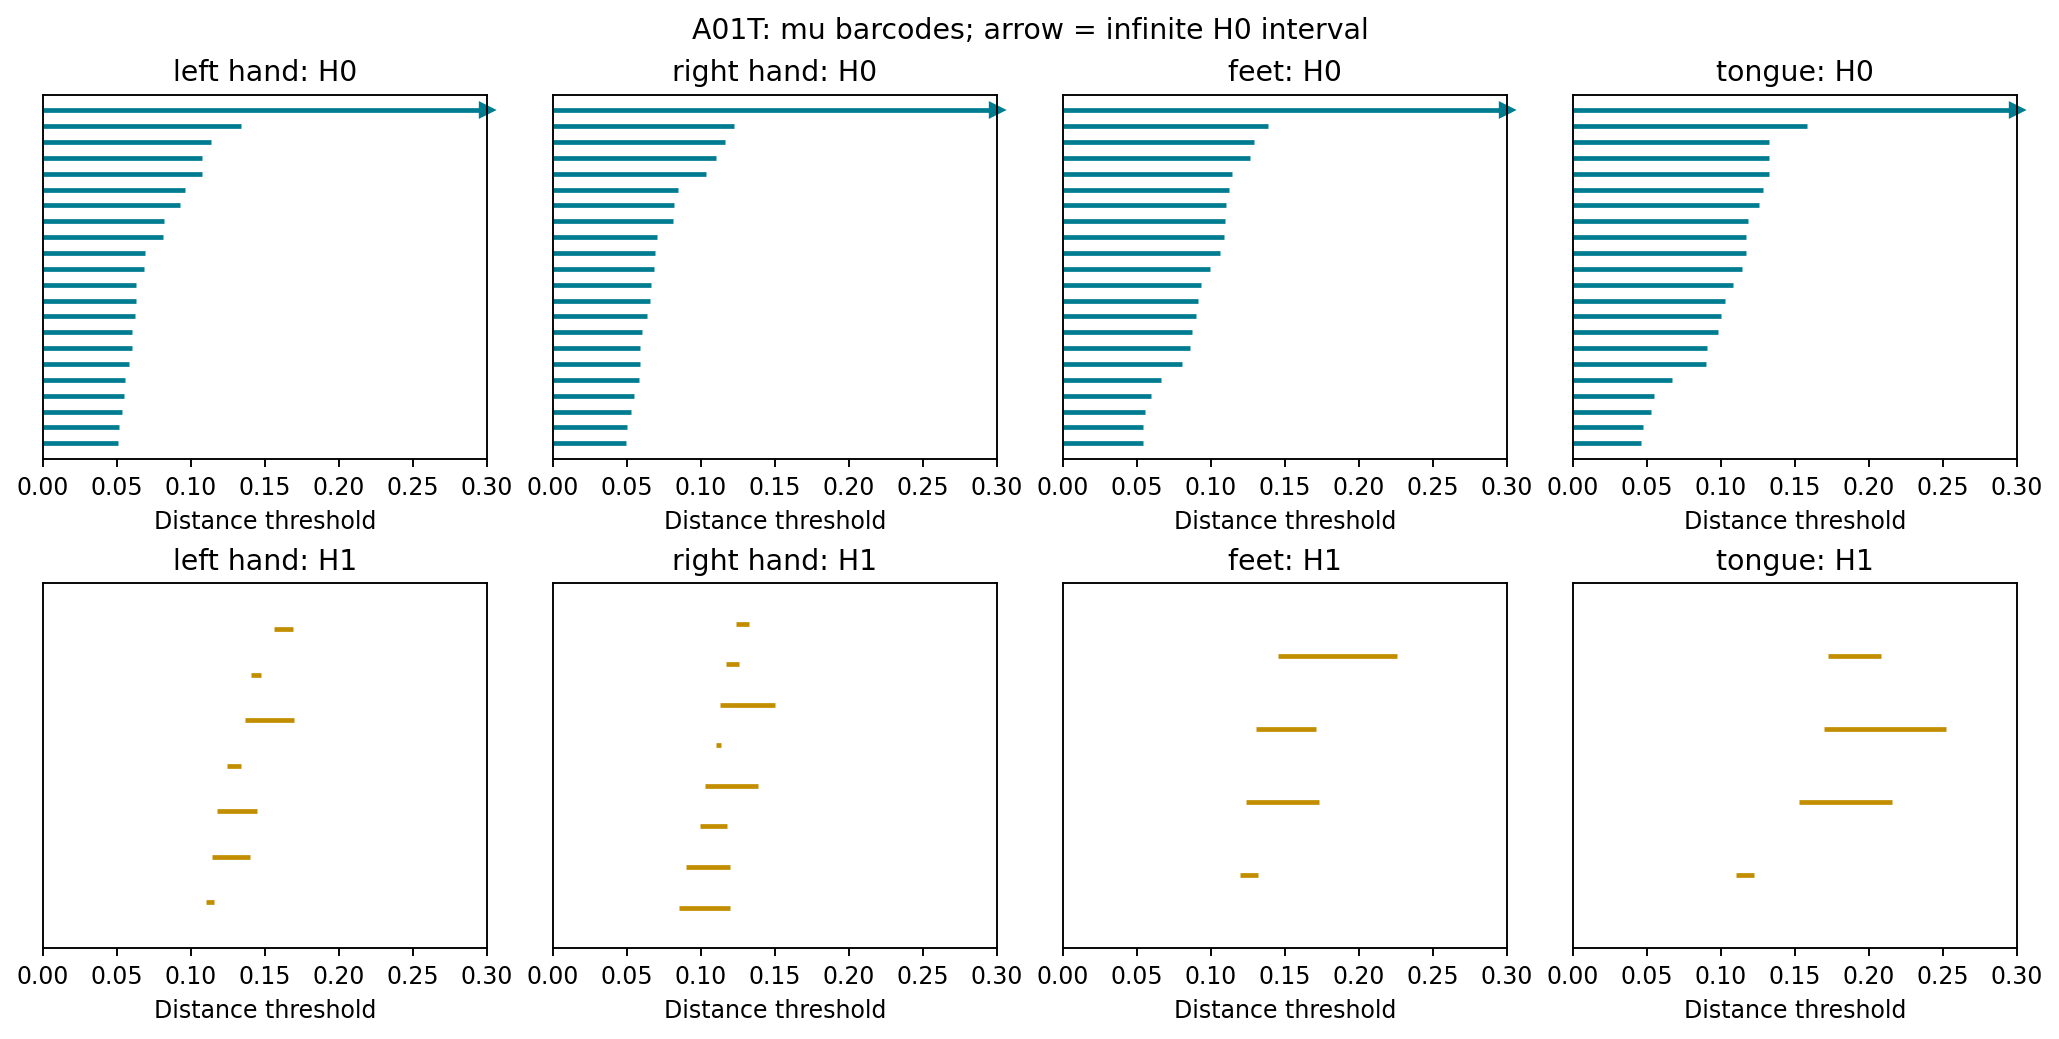
\includegraphics[width=\linewidth]{A01_barcodes_mu.png}
\caption{A01 mu-band barcodes for the seed-42 balanced selection (67 trials per movement). The arrow marks the essential $H_0$ interval. Blue/ochre lines encode threshold intervals, not EEG waveforms. The feet and tongue $H_1$ barcodes have fewer but longer-lived loops than the hand barcodes.}\label{fig:a01}
\end{figure}

\subsection{Differences across participants}
The A01 separation was not representative of every participant (Figure~\ref{fig:allnine}). For example, several participants' mu $H_0$ curves overlap closely, while A06 has generally larger merge thresholds and A02 smaller thresholds. These subject-level differences motivate paired, within-participant comparisons.

\begin{figure}[htbp]
\centering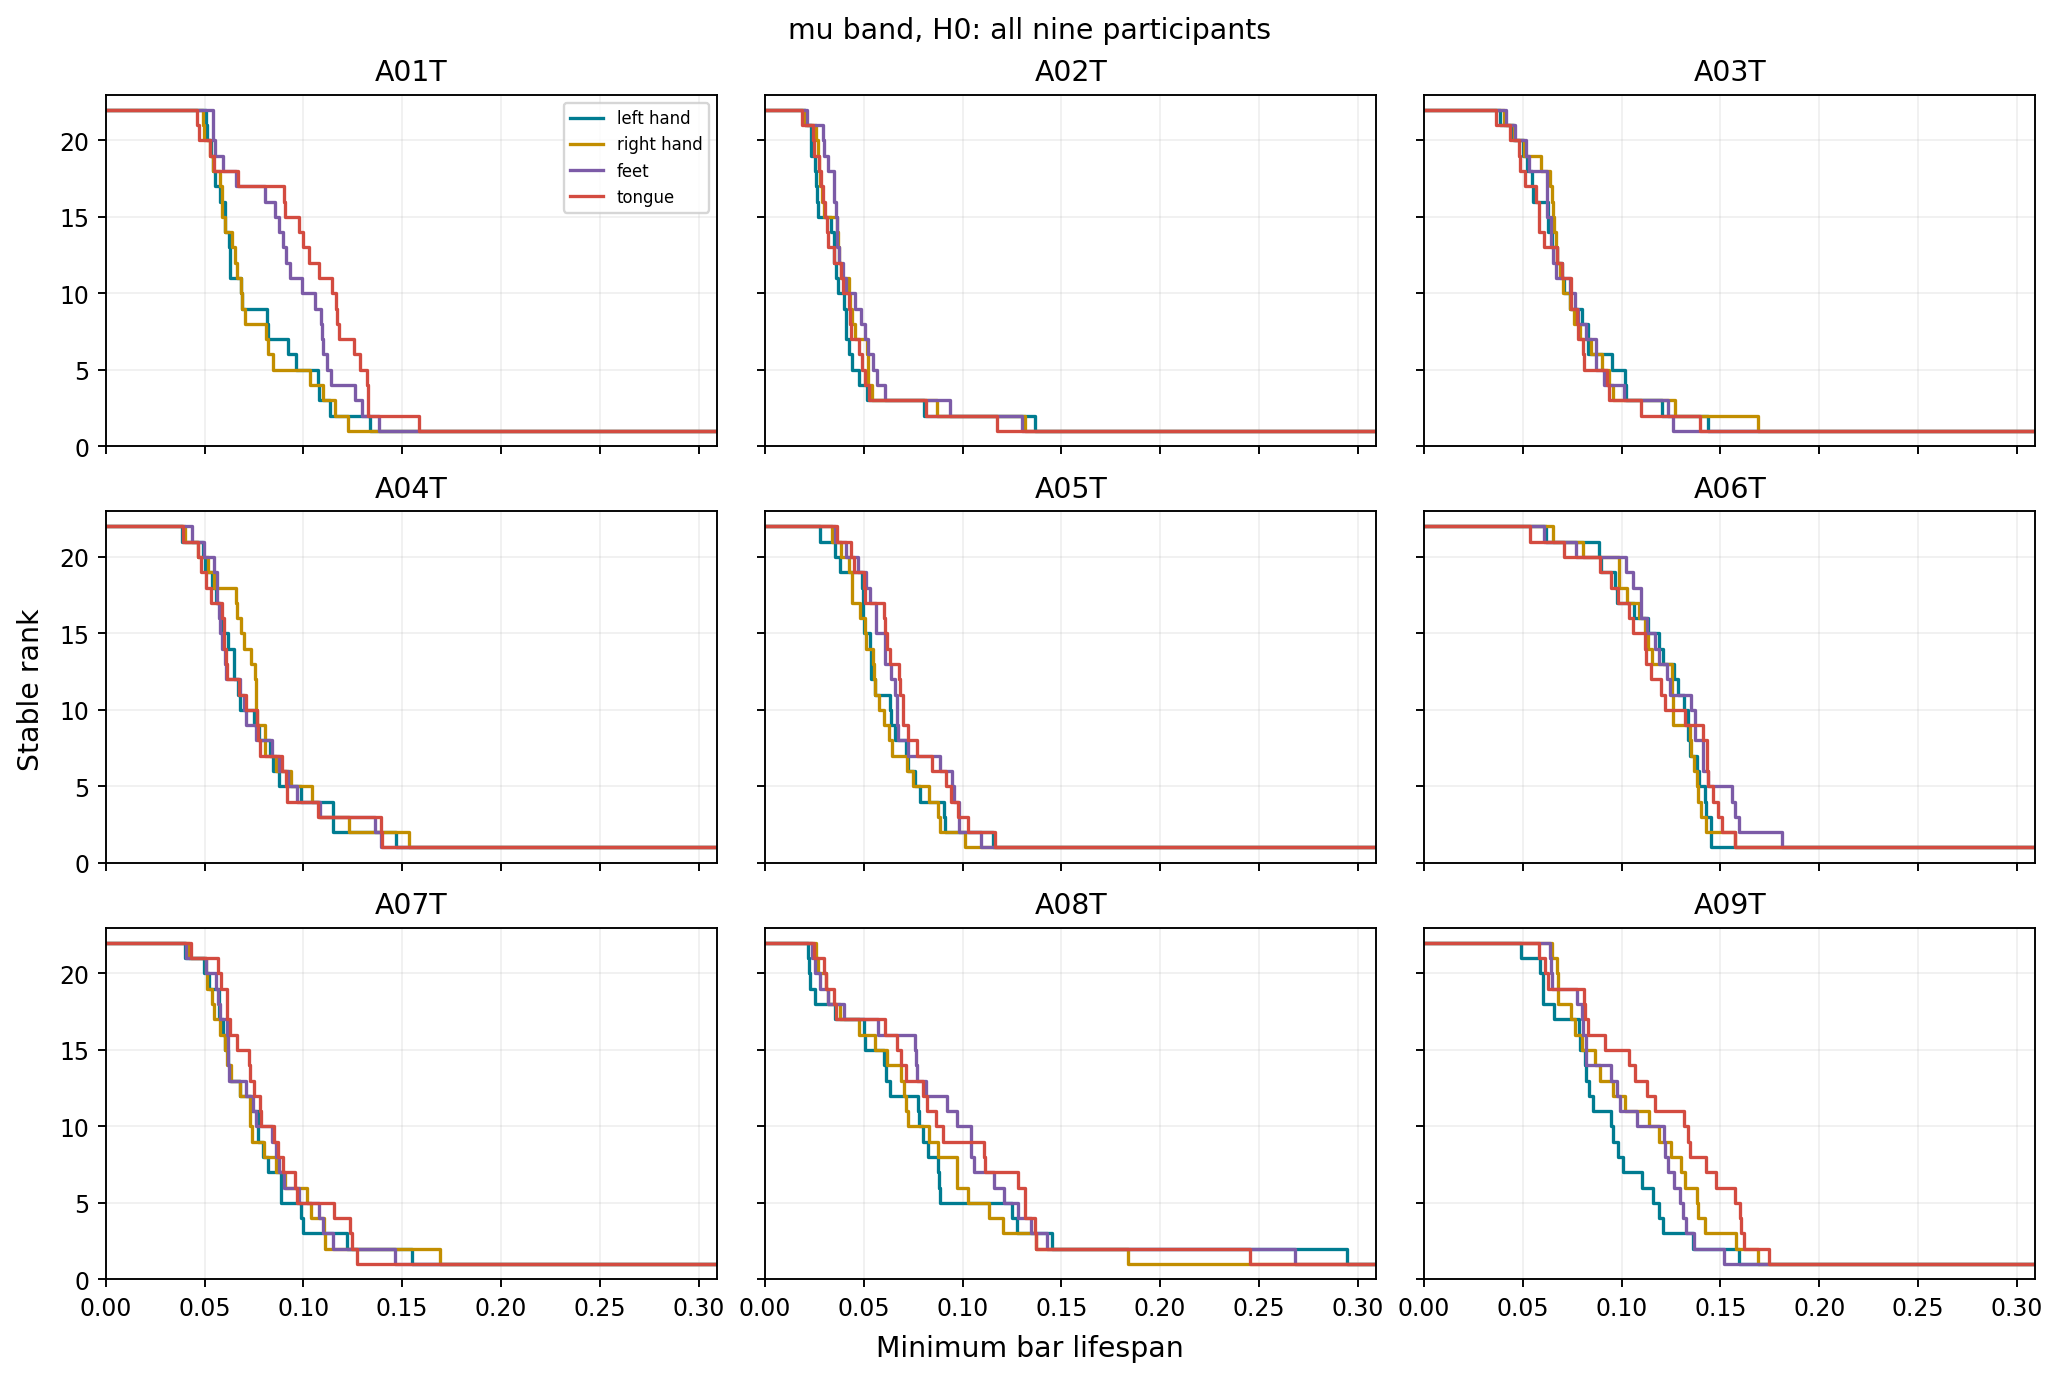
\includegraphics[width=\linewidth]{all_subjects_mu_H0.png}
\caption{Mu-band $H_0$ stable ranks for all nine participants on common axes. Colors have the same meaning in every panel. Movement differences and overall threshold scales vary between participants. The persistent level of one comes from the essential connected component.}\label{fig:allnine}
\end{figure}

Across participants, the median within-person mu $H_0$ L1 distance was 0.0822 for left versus right hand, compared with 0.1771 for left hand versus tongue and 0.1906 for right hand versus tongue (Figure~\ref{fig:l1}). These are descriptive separations of curves, not probabilities or test statistics. A larger distance does not indicate which movement has greater persistence.

The descriptive feet/tongue-minus-hands contrast in finite $H_0$ total persistence was positive in 7 of 9 participants in each band. Its median was 0.0713 in mu and 0.1008 in beta. For $H_1$, the direction was less consistent: positive in 5 of 9 participants in mu and 4 of 9 in beta. This contrast was motivated by A01 and is reported without a confirmatory significance claim.

\begin{figure}[htbp]
\centering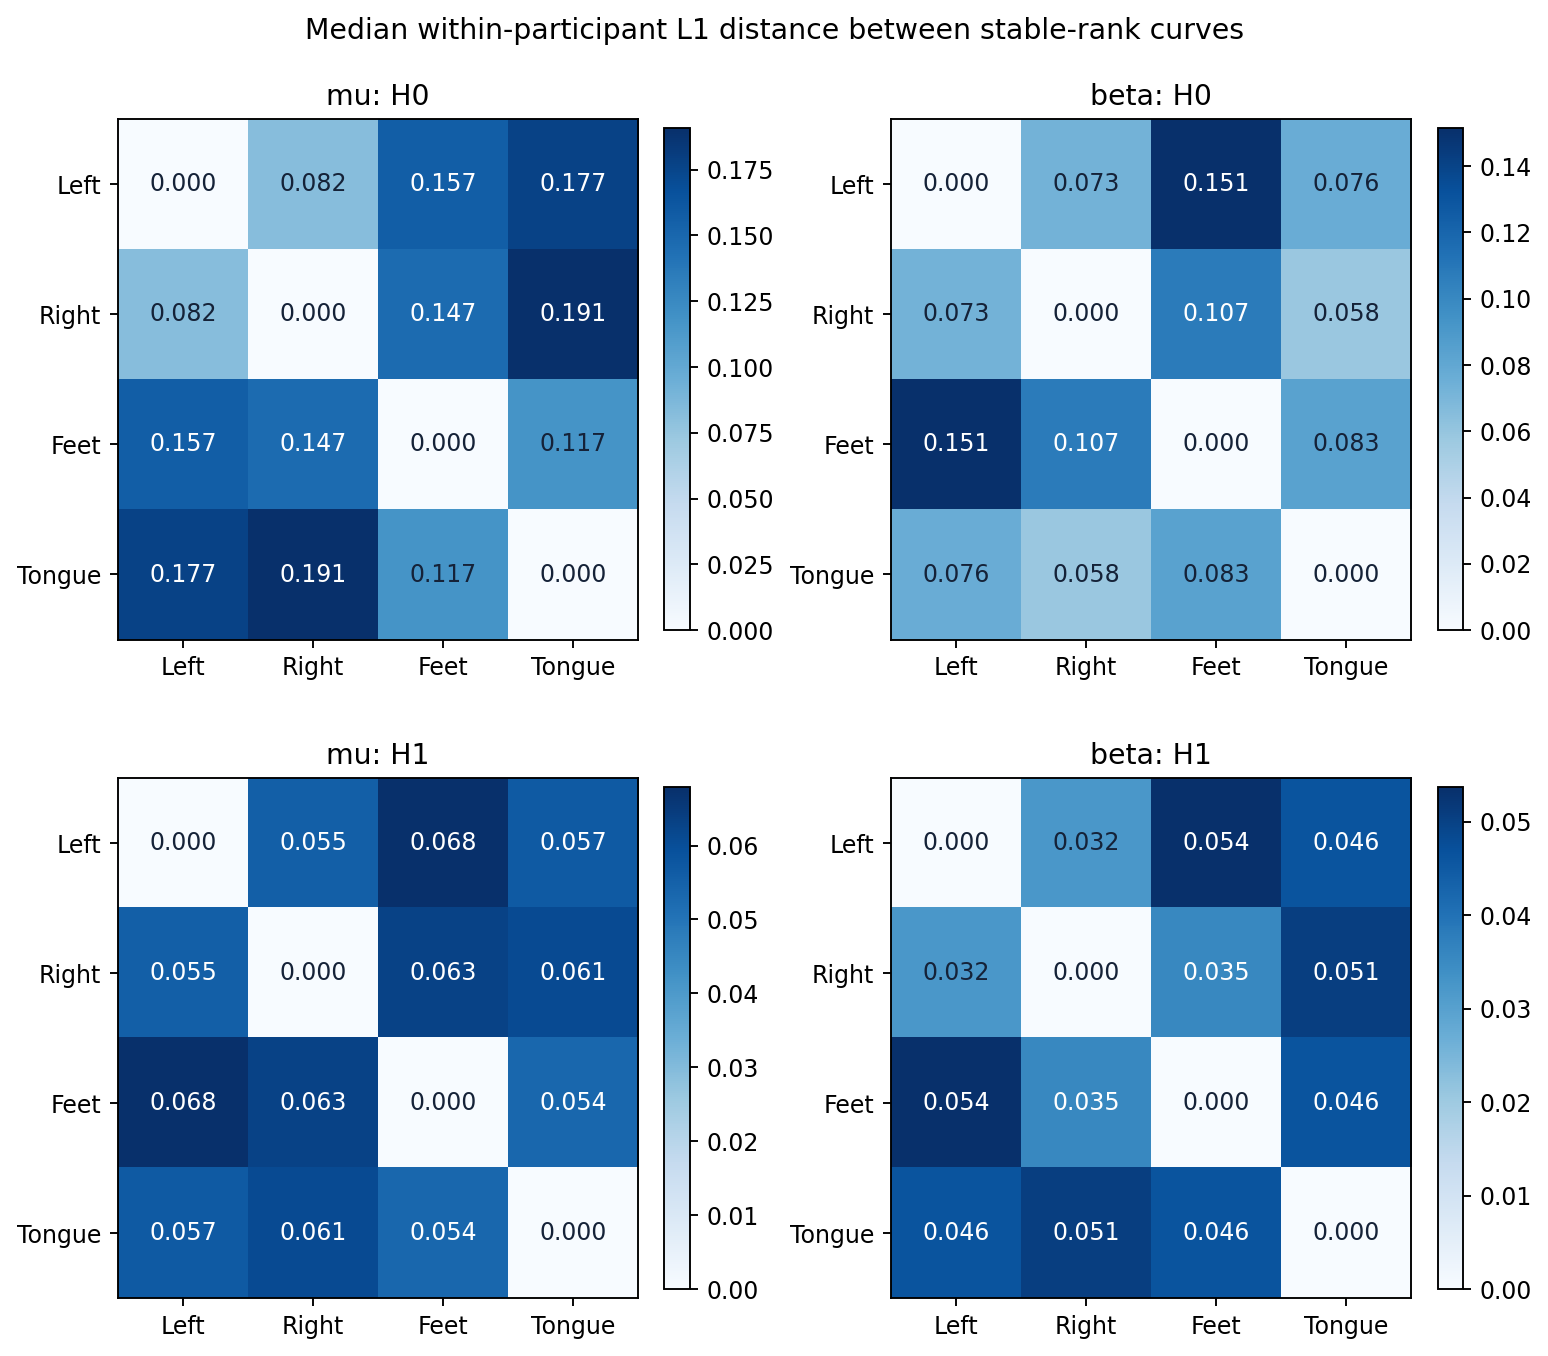
\includegraphics[width=0.83\linewidth]{group_pairwise_distances.png}
\caption{Across-participant medians of exact within-participant L1 distances between movement stable ranks. The four panels have separate color scales; comparisons must use the numbers. Zero diagonals compare each movement with itself. These are $4\times4$ movement comparisons, not channel matrices.}\label{fig:l1}
\end{figure}


\begin{table}[htbp]\centering

\caption{Median finite total persistence across nine participants; values are dimensionless. The infinite $H_0$ interval is excluded only from this scalar summary.}\label{tab:medians}

\begin{tabular}{llrrrr}\toprule

Band & Dimension & Left hand & Right hand & Feet & Tongue\\\midrule

Mu & $H_0$ & 1.5827 & 1.6236 & 1.6557 & 1.7327 \\

Mu & $H_1$ & 0.2489 & 0.2040 & 0.2166 & 0.2182 \\

Beta & $H_0$ & 2.2198 & 2.2375 & 2.2814 & 2.2935 \\

Beta & $H_1$ & 0.4086 & 0.3888 & 0.4016 & 0.3791 \\

\bottomrule\end{tabular}\end{table}

Table~\ref{tab:medians} and Figure~\ref{fig:paired} show that the central movement differences are modest relative to variation between participants. Medians of individual condition values need not equal medians of paired condition differences. Beta $H_0$ values are generally larger than mu $H_0$ values here, but no formal mu-versus-beta hypothesis test was specified; the bands use different frequency sets.

\begin{figure}[htbp]
\centering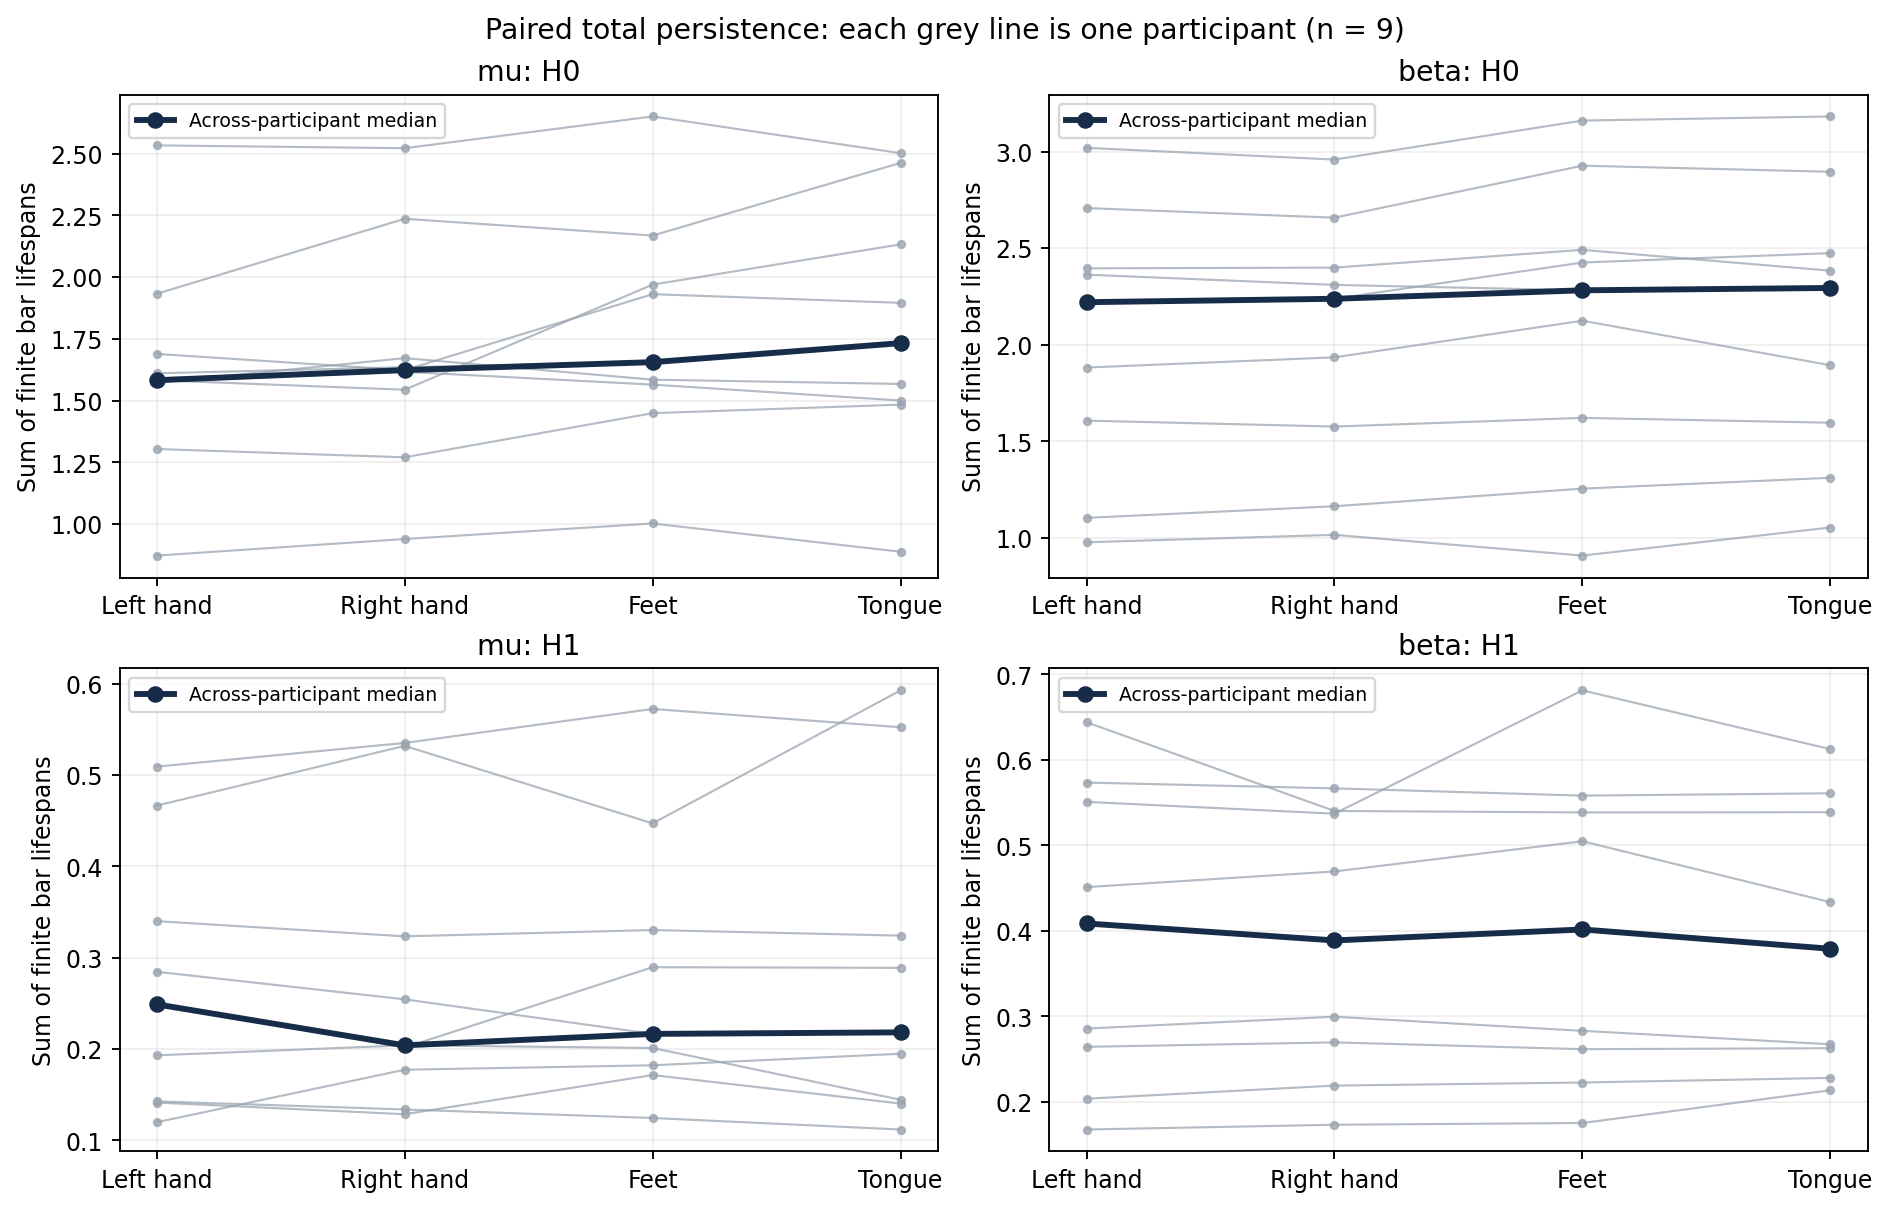
\includegraphics[width=\linewidth]{group_total_persistence.png}
\caption{Finite total persistence for the four movement conditions. Each grey line connects one participant's observations; the dark line is the pointwise median across participants. Curves that cross or change direction illustrate the inconsistent ordering of conditions.}\label{fig:paired}
\end{figure}

\subsection{Exploratory omnibus comparisons}
The four primary permutation tests did not detect a movement effect in finite total persistence after Holm adjustment (Table~\ref{tab:tests}). Rank agreement was low: Kendall's $W$ was about 0.160 for $H_0$ and 0.027--0.032 for $H_1$. This supports a cautious interpretation of the visual contrasts. A nonsignificant result does not prove that movements have identical networks or that the full stable-rank curves are equal: the tests use one finite-area summary and only nine participants.


\begin{table}[htbp]\centering

\caption{Exploratory primary tests of finite total persistence. Each test uses nine paired participants, four movement conditions and 99,999 within-participant label permutations.}\label{tab:tests}

\begin{tabular}{llrrrr}\toprule

Band & Dimension & Friedman $Q$ & Kendall $W$ & Permutation $p$ & Holm $p$\\\midrule

Mu & $H_0$ & 4.333 & 0.160 & 0.2455 & 0.9816 \\

Mu & $H_1$ & 0.867 & 0.032 & 0.8516 & 1.0000 \\

Beta & $H_0$ & 4.333 & 0.160 & 0.2454 & 0.9816 \\

Beta & $H_1$ & 0.733 & 0.027 & 0.8864 & 1.0000 \\

\bottomrule\end{tabular}\end{table}

Monte Carlo standard errors for the unadjusted primary $p$-values were approximately 0.0010--0.0014. This simulation uncertainty is small relative to their distance from 0.05. With 49 trials per movement for every participant (1,764 selected trials), the unadjusted $p$-values were 0.2901 (mu $H_0$), 0.7625 (mu $H_1$), 0.3053 (beta $H_0$) and 0.8184 (beta $H_1$); all four sensitivity-family Holm-adjusted values were 1.0000. Thus the absence of an omnibus signal in these summaries was unchanged by equalizing counts across participants.

\subsection{Sensitivity to trial selection and amplitude review}
All 180 repeated balanced selections completed. Table~\ref{tab:selection} summarizes exact L1 distances from the primary curve to each reselected curve, pooling the eight movement/band combinations and two homology dimensions within a participant. These pooled summaries are only a compact check; the separate curves and values are saved. A06 and A09 were more sensitive than the other participants. Their variation can be comparable with some movement-pair distances, so a small visual separation should not automatically be interpreted as a reliable movement signature.


\begin{table}[htbp]\centering

\caption{L1 change from the primary stable rank under 20 reselected balanced sets; each participant contributes 320 comparisons. These are sensitivity summaries, not confidence limits.}\label{tab:selection}

\begin{tabular}{lrr}\toprule Participant & Median change & Maximum change\\\midrule

A01T & 0.0053 & 0.0358 \\

A02T & 0.0043 & 0.0673 \\

A03T & 0.0043 & 0.0286 \\

A04T & 0.0096 & 0.0481 \\

A05T & 0.0068 & 0.0280 \\

A06T & 0.0237 & 0.1204 \\

A07T & 0.0063 & 0.0312 \\

A08T & 0.0054 & 0.0429 \\

A09T & 0.0210 & 0.1027 \\

\bottomrule\end{tabular}\end{table}

The amplitude rule identified nine review candidates: one in A01, two in A02 and six in A07. Removing these candidates temporarily changed only the conditions containing them. A01's tongue mu matrix changed by 0.001509 on average across unique channel pairs, with a maximum of 0.006213; its tongue beta changes were 0.000843 and 0.002298. The largest pairwise change anywhere in this check was 0.010402 (A02 tongue mu). The largest matrix mean change was 0.001740 (A02 tongue beta). Other participants had no additional amplitude-review exclusions in this scenario, giving zero changes by construction. These relatively small matrix changes do not establish artifact-free data or guarantee unchanged topological features; persistence was not recomputed for this amplitude-removal scenario.
